\documentclass[aspectratio=169, 22pt]{beamer}

\makeatletter
%\def\input@path{{../}{examples/}}
% When theme as submodule use the below line instead
\def\input@path{{usyd-beamer-theme/}}
\makeatother

\usepackage{tikz}
\usepackage{minted}
\usepackage{multicol}
\usepackage{subcaption}
\makeatletter
\let\@@magyar@captionfix\relax
\makeatother
\setlength{\columnseprule}{0.4pt}

\usepackage{amsmath}

\title{GPU-Accelerated Jump Flooding Algorithm for Voronoi Diagram in $log\star(n)$}
\subtitle{JFA$\star$, OpenCL}
\date{\today}
\author[M.A.C.]{Maciej A. Czyzewski}

\usetheme{usyd}
% To use the logobar theme use the line below instead
% \usetheme[logobar]{usyd}

\graphicspath{{./}}

%\titlegraphic{figure_3d}
\titlegraphic{jfa_star_intro2}
\titlegraphicbackground{usydwhite}

% FIXME: what we propose

% FIXME: wady metody JFA -->?????????

% FIXME: spotrzezenia --> czarne miejsca brakujaca informacja
% FIXME: postrzzenia  --> 9 kwadratow ma swoja wade --> lepszy okrag
% FIXME: ilosc krokow --> dla losowej maski nie musi juz byc log 2**n

\begin{document}

%%%%%%%%%%%%%%%%%%%%%%%%%%%%%%%%%%%%%%%%%%%%%%%%%%%%%%%%%%%%%%%%%%%%%%%%%%%%%%%%

\begin{frame}
  \titlepage{}
\end{frame}

%%%%%%%%%%%%%%%%%%%%%%%%%%%%%%%%%%%%%%%%%%%%%%%%%%%%%%%%%%%%%%%%%%%%%%%%%%%%%%%%

\begin{frame}{Our $log\star(n)$ vs. Current $log(p)$ \\
	(where $n$ - seeds in
	diagram, $p$ - resolution in
	pixels)}

\begin{figure}
\centering
\begin{subfigure}{.5\textwidth}
  \centering
  \includegraphics[width=1\linewidth]{./figure_jka_star.png}
	\caption{JFA$\star$+1 (4 steps)}
  \label{fig:sub1}
\end{subfigure}%
\begin{subfigure}{.5\textwidth}
  \centering
  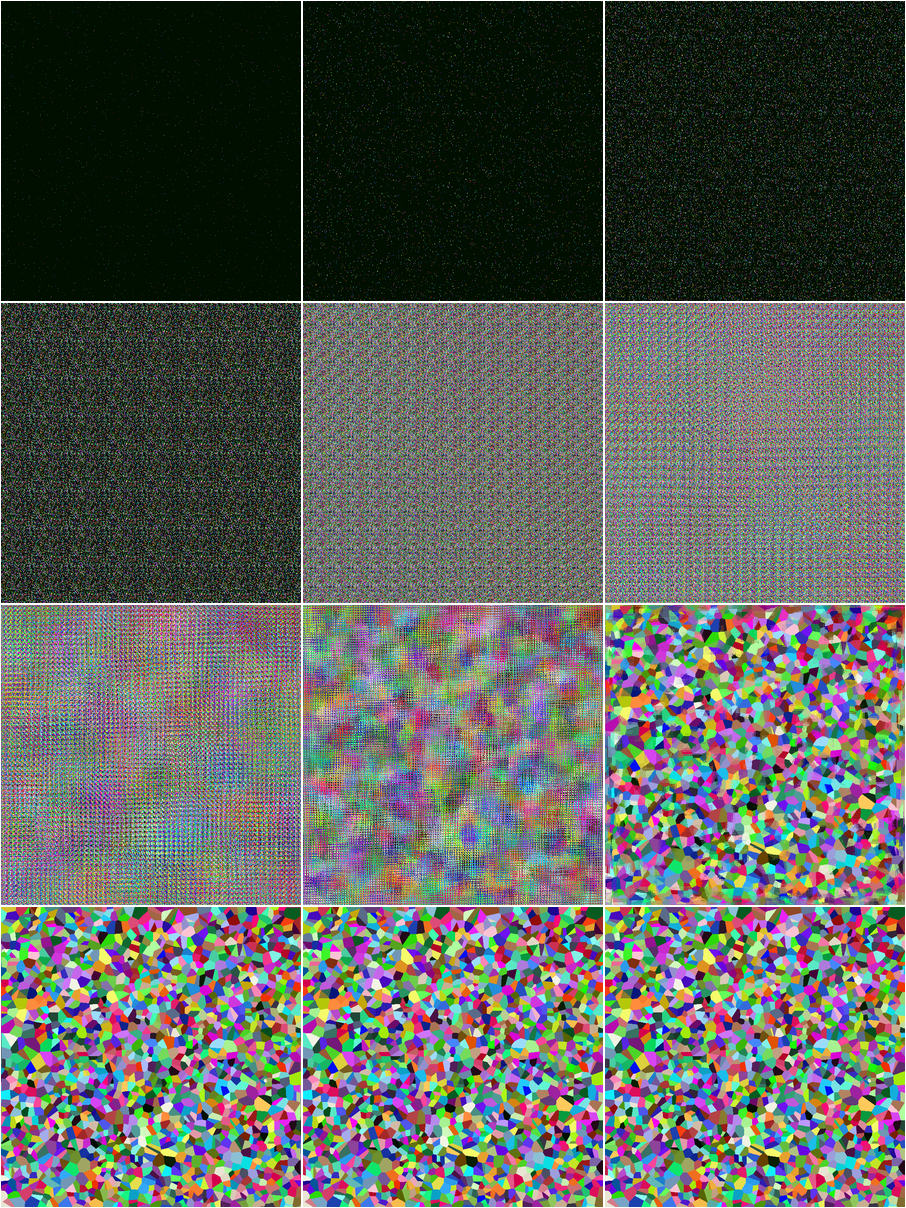
\includegraphics[width=0.5\linewidth]{./figure_jka.png}
	\caption{JFA+1 (10 steps)}
  \label{fig:sub2}
\end{subfigure}
	\caption{$\text{x}=720; \text{y}=720; \text{seeds}=2000$
	  (read as $\text{n}=2000; \text{p}=720$).}
\label{fig:test}
\end{figure}

\end{frame}

%%%%%%%%%%%%%%%%%%%%%%%%%%%%%%%%%%%%%%%%%%%%%%%%%%%%%%%%%%%%%%%%%%%%%%%%%%%%%%%%

\begin{frame}

\begin{figure}
\centering
\includegraphics[width=0.65\linewidth]{./figure_3d.png}
\label{fig:test}
\end{figure}

\end{frame}

%%%%%%%%%%%%%%%%%%%%%%%%%%%%%%%%%%%%%%%%%%%%%%%%%%%%%%%%%%%%%%%%%%%%%%%%%%%%%%%%

\begin{frame}

\begin{figure}
\centering
\begin{subfigure}{.5\textwidth}
  \centering
  \includegraphics[width=0.7\linewidth]{./figure_seed_8.png}
  \label{fig:sub1}
\end{subfigure}%
\begin{subfigure}{.5\textwidth}
  \centering
  \includegraphics[width=0.7\linewidth]{./figure_seed_64.png}
  \label{fig:sub2}
\end{subfigure}
\begin{subfigure}{.5\textwidth}
  \centering
  \includegraphics[width=0.7\linewidth]{./figure_seed_1024.png}
  \label{fig:sub2}
\end{subfigure}%
\begin{subfigure}{.5\textwidth}
  \centering
  \includegraphics[width=0.7\linewidth]{./figure_seed_65536.png}
  \label{fig:sub2}
\end{subfigure}
\label{fig:test}
\end{figure}

\end{frame}

%%%%%%%%%%%%%%%%%%%%%%%%%%%%%%%%%%%%%%%%%%%%%%%%%%%%%%%%%%%%%%%%%%%%%%%%%%%%%%%%

\begin{frame}[fragile]{JFA: classic approach on GPU}

\vspace{-1em}
\begin{multicols}{2} % small, footnotesize
\begin{minted}[tabsize=2,fontsize=\footnotesize]{C++}
int gid = get_global_id(0);
int y =  gid    % Y_size;
int x = (gid-y) / X_size;
#define POS(X, Y) ((X)*X_size + (Y))

int best_0  = M_g[ gid], // input
    best_1a = P1_g[gid],
    best_1b = P2_g[gid];
float bestS = metric(best_1a, best_1b,
                           x,       y);
if (best_0 == 0)
	bestS = 4294967296; // +inf

int pos[] = {-step, 0, step};

// SELECTION //////////////////////////
for(int i = 0; i < 3; i++) // problem #2
for(int j = 0; j < 3; j++) {
	int idx = POS(x+pos[i], y+pos[j]);
	if (P1_g[idx] == 0 && \ // problem #1
	    P2_g[idx] == 0) continue;
	float s2 = metric(
		P1_g[idx], P2_g[idx], x, y);
	if (bestS >= s2) {
		best_0  = M_g[ idx];
		best_1a = P1_g[idx];
		best_1b = P2_g[idx];
		bestS   = s2;
	}}
///////////////////////////////////////

M_o[ gid] =  best_0; // output
P1_o[gid] = best_1a;
P2_o[gid] = best_1b;
\end{minted}
\end{multicols}

\end{frame}

%%%%%%%%%%%%%%%%%%%%%%%%%%%%%%%%%%%%%%%%%%%%%%%%%%%%%%%%%%%%%%%%%%%%%%%%%%%%%%%%

\begin{frame}{Problem \#1: wasting time in empty areas}

\begin{tikzpicture}
	\node[anchor=south west,inner sep=0] (no) at (-2,0,0)
	{\includegraphics[width=0.25\linewidth]{./no.png}};

	\node[anchor=south west,inner sep=0] (image) at (0,0,0)
	{\includegraphics[width=0.5\linewidth]{./jfa_no_data.png}};
    \begin{scope}[x={(image.south east)},y={(image.north west)}]
        \draw[dashed,-latex,red] (0.8,0.8) -- +(1.1in,0.2in)node[anchor=west]
		{no data!};
        \draw[dashed,-latex,red] (0.6,0.6) -- +(1.9in,0)node[anchor=west] {no
		data!};
        \draw[dashed,-latex,red] (0.4,0.5) -- +(-2in,+1in)node[anchor=east] {no
		data!};
        \draw[dashed,-latex,red] (0.5,0.4) -- +(-2.4in,-0.5in)node[anchor=east] {no data!};
    \end{scope}
\end{tikzpicture}

\end{frame}

%%%%%%%%%%%%%%%%%%%%%%%%%%%%%%%%%%%%%%%%%%%%%%%%%%%%%%%%%%%%%%%%%%%%%%%%%%%%%%%%

\begin{frame}{Solution \#1: apply random noise}

\begin{tikzpicture}
	\node[anchor=south west,inner sep=0] (no) at (-2,0,0)
	{\includegraphics[width=0.25\linewidth]{./yes.png}};

	\node[anchor=south west,inner sep=0] (image) at (0,0,0)
	{\includegraphics[width=0.5\linewidth]{./noise.png}};
    \begin{scope}[x={(image.south east)},y={(image.north west)}]
        \draw[dashed,-latex,green] (0.8,0.8) -- +(1.1in,0.2in)node[anchor=west]
		{data!};
        \draw[dashed,-latex,green] (0.6,0.6) -- +(1.9in,0)node[anchor=west]
		{data!};
        \draw[dashed,-latex,green] (0.4,0.5) -- +(-2in,+1in)node[anchor=east]
		{\qquad data!};
        \draw[dashed,-latex,green] (0.5,0.4) --
		+(-2.4in,-0.5in)node[anchor=east] {\qquad data!};
    \end{scope}
\end{tikzpicture}

\end{frame}

%%%%%%%%%%%%%%%%%%%%%%%%%%%%%%%%%%%%%%%%%%%%%%%%%%%%%%%%%%%%%%%%%%%%%%%%%%%%%%%%

\begin{frame}{Solution \#1: apply random noise (why?)}
\begin{columns}
\column{0.5\linewidth}
	\includegraphics[width=1\linewidth]{./lazy_clouds.png}%
\column{0.5\linewidth}

\begin{enumerate}
\item In areas where the classic JFA does not perform any calculations,
	JFA$\star$ performs \textbf{passive grouping} (noise reduction), often on the
	correct seeds, therefore small corrections are needed in the next steps
\item In this way, the same algorithm behaves like as if performing
	weighted \underline{quick-union} with path compression. Therefore, in a smaller number of steps, the result is obtained
\end{enumerate}

\end{columns}
\end{frame}

%%%%%%%%%%%%%%%%%%%%%%%%%%%%%%%%%%%%%%%%%%%%%%%%%%%%%%%%%%%%%%%%%%%%%%%%%%%%%%%%

\begin{frame}[fragile]{Solution \#1: noise in-place (JFA$+$)}

\vspace{-1em}
\begin{multicols}{2} % small, footnotesize
\begin{minted}[tabsize=2,fontsize=\footnotesize]{C++}
// SELECTION //////////////////////////
for(int i = 0; i < 3; i++)
for(int j = 0; j < 3; j++) {
	int idx = POS(x+pos[i], y+pos[j]);
	int m  = M_g[ idx], // current
	    p1 = P1_g[idx],
	    p2 = P2_g[idx];
	// if no information, get from noise
	if (p1 == 0 && p2 == 0) {
		int ridx = NOISE_g[idx];
		m  = IDS_g[ridx];
		p1 = PTS_g[ridx].x;
		p2 = PTS_g[ridx].y;
	}
	float s2 = metric(p1, p2, x, y);
	if (bestS >= s2) {
		best_0  = m;
		best_1a = p1;
		best_1b = p2;
		bestS   = s2;
	}}
///////////////////////////////////////
\end{minted}
\end{multicols}

\end{frame}

%%%%%%%%%%%%%%%%%%%%%%%%%%%%%%%%%%%%%%%%%%%%%%%%%%%%%%%%%%%%%%%%%%%%%%%%%%%%%%%%

\begin{frame}[fragile]{Solution \#1: applying mask with noise (JFA$\star$)}

\vspace{-1em}
\begin{multicols}{2} % small, footnotesize
\begin{minted}[tabsize=2,fontsize=\large]{C++}
int gid = get_global_id(0);
int m  = M_g[ gid],
    p1 = P1_g[gid],
    p2 = P2_g[gid];

// if no information,
//     get from noise
if (p1 == 0 && p2 == 0) {
	int ridx = NOISE_g[gid];
	m  = IDS_g[ridx];
	p1 = PTS_g[ridx].x;
	p2 = PTS_g[ridx].y;
}


M_o[ gid] =  m; // output
P1_o[gid] = p1;
P2_o[gid] = p2;
\end{minted}
\end{multicols}

\end{frame}

%%%%%%%%%%%%%%%%%%%%%%%%%%%%%%%%%%%%%%%%%%%%%%%%%%%%%%%%%%%%%%%%%%%%%%%%%%%%%%%%

\begin{frame}{Problem \#2: selection is too regular}

\begin{figure}
\centering
\includegraphics[width=0.40\linewidth]{./problem_2.png}
\label{fig:test}
\caption{A Voronoi cell shown partially as a wedge can ``steal'' a center
pixel $p$ without including any of the eight neighboring pixels. Such a
	Voronoi cell looks disconnected when displayed on screen. [Guodong 2006]}
\end{figure}

\end{frame}

%%%%%%%%%%%%%%%%%%%%%%%%%%%%%%%%%%%%%%%%%%%%%%%%%%%%%%%%%%%%%%%%%%%%%%%%%%%%%%%%

\begin{frame}{Solution \#2: random points in circle}


\begin{figure}
\centering
\includegraphics[width=0.82\linewidth]{./circle_random.jpg}
\label{fig:test}
\caption{The solution to this problem is to select points on a circle during
	each step. In this figure, it can be seen that thanks to that we can choose
	the area of interest (i.e. $r_{i+i}$).}
\end{figure}

\end{frame}

%%%%%%%%%%%%%%%%%%%%%%%%%%%%%%%%%%%%%%%%%%%%%%%%%%%%%%%%%%%%%%%%%%%%%%%%%%%%%%%%

\begin{frame}{Solution \#2: the difference at the same step}

\begin{figure}
\centering
\begin{subfigure}{.5\textwidth}
  \centering
  \includegraphics[width=0.75\linewidth]{./solution_2a.png}
	\caption{JFA$\star$+1 (circle: random 12 points)}
  \label{fig:sub1}
\end{subfigure}%
\begin{subfigure}{.5\textwidth}
  \centering
  \includegraphics[width=0.75\linewidth]{./solution_2b.png}
	\caption{JFA+1 (grid: regular 9 points)}
  \label{fig:sub2}
\end{subfigure}
	\caption{Please note that Voronoi cells are already clearly defined in our
	method.}
\label{fig:test}
\end{figure}

\end{frame}

%%%%%%%%%%%%%%%%%%%%%%%%%%%%%%%%%%%%%%%%%%%%%%%%%%%%%%%%%%%%%%%%%%%%%%%%%%%%%%%%

\begin{frame}{Solution \#2: difference in entropy}

\begin{figure}
\centering
\begin{subfigure}{.3\textwidth}
  \centering
  \includegraphics[width=0.8\linewidth]{./zoom2.png}
	\caption{JFA$\star$+1}
  \label{fig:sub1}
\end{subfigure}%
\begin{subfigure}{.3\textwidth}%
  \centering
  \includegraphics[width=0.8\linewidth]{./zoom1.png}
	\caption{JFA+1}
  \label{fig:sub2}
\end{subfigure}
\begin{subfigure}{.3\textwidth}
  \centering
  \includegraphics[width=0.8\linewidth]{./zoomf.png}
	\caption{Voronoi}
  \label{fig:sub2}
\end{subfigure}

	\caption{The difference presented above in for these methods.}
\label{fig:test}
\end{figure}

\end{frame}

%%%%%%%%%%%%%%%%%%%%%%%%%%%%%%%%%%%%%%%%%%%%%%%%%%%%%%%%%%%%%%%%%%%%%%%%%%%%%%%%

\begin{frame}{Question \#1: how many steps do we need now?}

\centering\textbf{I DON'T NOW!} \\
no mathematical proof

\end{frame}

%%%%%%%%%%%%%%%%%%%%%%%%%%%%%%%%%%%%%%%%%%%%%%%%%%%%%%%%%%%%%%%%%%%%%%%%%%%%%%%%

\begin{frame}{Question \#1: empirical observations}

%               JFA$\star$          JFA$+$        JFA
% impro.       noise+selection     noise           --
% step num.    log$\star$(n)      log4(p)       log2(p)
% step size   p / (3**(i)))   p / (2**(i)))  p / (2**(i)))

\Large
\centering
\begin{tabular}{ l|c|c|c }

			 &  JFA$\star$        &  JFA$+$    &    JFA         \\ \hline
	used improvement      & noise+selection &    noise   &        --        \\
	num. of needed steps  &  log$\star$(n)  &    log4(p)  &     log2(p)      \\
	step size &  $\frac{p}{3^i}$ &  $\frac{p}{2^i}$ & $\frac{p}{2^i}$  \\

\end{tabular}

\end{frame}

%%%%%%%%%%%%%%%%%%%%%%%%%%%%%%%%%%%%%%%%%%%%%%%%%%%%%%%%%%%%%%%%%%%%%%%%%%%%%%%%

\begin{frame}{Recommended reading}

\begin{enumerate}
\item ``Jump Flooding in GPU with Applications to Voronoi Diagram and Distance
	Transform'', Guodong Rong, Tiow-Seng Tan, 2006
\item ``Facet-JFA: Faster computation of discrete Voronoi diagrams'', Talha Bin
	Masoodi, Hari Krishna Malladi, Vijay Natarajan, 2014
\end{enumerate}

\end{frame}

\end{document}
